% Provenance (never printed): cycle 4 SVT, "La planete Terre, l'environnement
% et l'action humaine": natural risks, hazard and vulnerability, prevention
% and protection; see sources/book1/PROVENANCE.md. Book 1, grade 9, chapter 2.
% Vocabulary guard: owns risk, vulnerability, prevention, hazard map.
% Natural hazard and natural disaster, the warning colours and the safety
% rules are g5's (natural-hazards); the warning signs of an eruption and the
% Pinatubo story are g7's (volcanoes); seismometer, tsunami and "scientists
% cannot predict earthquakes" are g7's (earthquakes); flood and floodplain
% are g5's (water-shapes-the-land); weather forecast is g8's. Lahars are
% called mudflows (as in g7). "Normal fault" is Book 2's: here "a fault".
\chapter{प्राकृतिक जोखिमों के साथ जीना}\label{ch:g9:natural-risks}

13~नवंबर 1985 की देर शाम, कोलंबिया के एक कस्बे आर्मेरो के ज़्यादातर लोग बिस्तर में थे।
एक \omterm{def:g5:natural-hazards:storm}{तूफ़ान} ने \qty{45}{km} दूर के बर्फ़ से ढके \omterm{def:g4:volcanoes-earthquakes-first-look:volcano}{ज्वालामुखी} नेवाडो देल रुइज़ को ढक रखा
था, और कस्बे में किसी ने उसे फटते नहीं देखा। गरम \omterm{def:g3:stones-pebbles-sand:rock}{चट्टानों} ने उसकी बर्फ़ का एक हिस्सा
पिघला दिया, और राख और \omterm{def:g3:stones-pebbles-sand:rock}{चट्टान} से मिला पानी कीचड़ प्रवाहों के रूप में \omterm{def:g1:landscapes-around-us:landform}{घाटियों} में नीचे दौड़ा।
लगभग दो घंटे बाद कीचड़ प्रवाह लागुनियास \omterm{def:g1:landscapes-around-us:water}{नदी} की \omterm{def:g1:landscapes-around-us:landform}{घाटी} से निकलकर सीधे कस्बे में घुस गए:
कोई \num{23000} लोग, कस्बे के ज़्यादातर लोग, मारे गए। दो घंटे ऊँची ज़मीन तक पैदल जाने
के लिए काफ़ी समय था। आर्मेरो के लोगों को बताया नहीं गया
था।
% ledger: usgs:armero

\begin{omfigure}
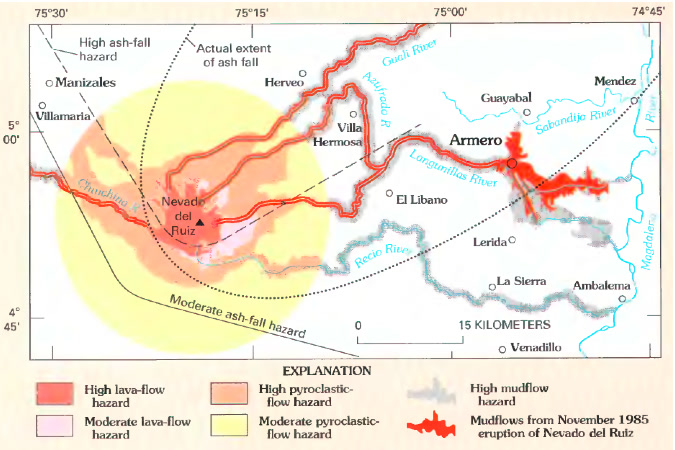
\includegraphics[width=0.86\linewidth]{images/book1/g9-ruiz-hazard-map.jpg}

{\small नेवाडो देल रुइज़ का \omterm{def:g9:natural-risks:hazard-map}{संकट मानचित्र}। कोलंबियाई भूवैज्ञानिकों का बनाया पहला संस्करण
\omterm{def:g4:volcanoes-earthquakes-first-look:eruption}{उद्गार} से एक महीना पहले बँट चुका था और आर्मेरो की \omterm{def:g1:landscapes-around-us:landform}{घाटी} में कीचड़ प्रवाहों का ख़तरा पहले
ही दिखाता था। यह संस्करण, आपदा के बाद फिर से बनाया गया, चटक लाल रंग में वे कीचड़ प्रवाह
जोड़ता है जो सच में नवंबर 1985 में आए (\omterm{def:g4:volcanoes-earthquakes-first-look:volcano}{ज्वालामुखी} के चारों ओर छायांकित वृत्त की त्रिज्या
लगभग \qty{20}{km} है)। राइट और पियर्सन, USGS सर्कुलर 1073, 1992 से
(सार्वजनिक डोमेन, विकिमीडिया कॉमन्स के
ज़रिए)।}
% ledger: usgs:ruiz-map, commons:ruiz-map
\label{fig:g9:natural-risks:ruiz}
\end{omfigure}

छह वर्ष बाद, फ़िलिपींस में माउंट पिनातूबो पर, \omterm{def:g4:volcanoes-earthquakes-first-look:volcano}{ज्वालामुखी} पर नज़र रखी गई, चेतावनी समय पर
आई और लोग वहाँ से चले गए (\cref{ch:g7:volcanoes})। दोनों विस्फोटक \omterm{def:g4:volcanoes-earthquakes-first-look:volcano}{ज्वालामुखी} थे, और
दोनों के कीचड़ प्रवाहों के रास्ते में लोग रहते थे। फ़र्क़ इसमें था कि लोग क्या जानते थे,
और उन्होंने उस जानकारी के साथ क्या किया। यह अध्याय उसी फ़र्क़ के बारे में
है।
% ledger: usgs:armero (Pinatubo 1991 averted a disaster like Armero), usgs:pinatubo-1991

\begin{recall}
\emph{\omterm{def:g5:natural-hazards:hazard}{प्राकृतिक संकट}} एक प्राकृतिक घटना है जो लोगों को नुक़सान पहुँचा सकती है; वह
\emph{\omterm{def:g5:natural-hazards:disaster}{प्राकृतिक आपदा}} बन जाती है जब वह वहाँ आए जहाँ लोग रहते हैं और भारी नुक़सान
करे (\cref{ch:g5:natural-hazards})। उफनती \omterm{def:g1:landscapes-around-us:water}{नदी} अपने \omterm{def:g5:water-shapes-the-land:flood}{बाढ़} के \omterm{def:g1:landscapes-around-us:landform}{मैदान} को ढक लेती है
(\cref{ch:g5:water-shapes-the-land})। बड़े \omterm{def:g4:volcanoes-earthquakes-first-look:eruption}{उद्गार} से पहले \omterm{def:g4:volcanoes-earthquakes-first-look:volcano}{ज्वालामुखी} अक्सर चेतावनी के
संकेत देता है: छोटे \omterm{def:g4:volcanoes-earthquakes-first-look:earthquake}{भूकंप}, फूलती ढलानें, गैस (\cref{ch:g7:volcanoes})। वैज्ञानिक
\omterm{def:g4:volcanoes-earthquakes-first-look:earthquake}{भूकंपों} की भविष्यवाणी नहीं कर सकते; \omterm{def:g7:earthquakes:seismometer}{भूकंपमापी} उन्हें दर्ज करते हैं, और \omterm{def:g2:water-on-earth:ocean}{समुद्र} के नीचे का
\omterm{def:g4:volcanoes-earthquakes-first-look:earthquake}{भूकंप} \omterm{def:g7:earthquakes:tsunami}{सुनामी} पैदा कर सकता है (\cref{ch:g7:earthquakes})। \omterm{def:g8:fronts-and-weather-maps:forecast}{मौसम पूर्वानुमान} बताता है कि
आने वाले दिनों में \omterm{def:g1:watching-the-weather:weather}{मौसम} कैसा रहेगा
(\cref{ch:g8:fronts-and-weather-maps})।
\end{recall}

\section{संकट, सुभेद्यता और जोखिम}

एक ही \omterm{def:g4:volcanoes-earthquakes-first-look:earthquake}{भूकंप} हर जगह एक-सा नुक़सान नहीं करता। किसी ख़ाली \omterm{def:g5:weather-and-climate:desert}{मरुस्थल} के नीचे वह किसी को
नुक़सान नहीं पहुँचाता। मज़बूत इमारतों वाले ऐसे कस्बे के नीचे जिसके लोग जानते हैं कि क्या
करना है, वह हिलाता है, डराता है और खिड़कियाँ तोड़ता है। भारी, ख़राब बने घरों वाले कस्बे के
नीचे वह उन्हें अंदर के लोगों पर गिरा सकता है। संकट वही है; जो बदलता है वह यह है कि जगह
को कितनी आसानी से नुक़सान पहुँच सकता
है।

\begin{definition}[सुभेद्यता]\label{def:g9:natural-risks:vulnerability}
किसी जगह की \emph{सुभेद्यता}\index{सुभेद्यता} यह है कि उसके लोगों, उसकी इमारतों
और उनकी ज़रूरत की चीज़ों को किसी \omterm{def:g5:natural-hazards:hazard}{प्राकृतिक संकट} से कितनी आसानी से नुक़सान पहुँच सकता है।
\omterm{def:g5:water-shapes-the-land:flood}{बाढ़} के \omterm{def:g1:landscapes-around-us:landform}{मैदान} पर घर, कमज़ोर इमारतें, कोई चेतावनी नहीं और कोई योजना नहीं, ये एक जगह को
सुभेद्य बनाते हैं।
\end{definition}

\begin{definition}[जोखिम]\label{def:g9:natural-risks:risk}
किसी \omterm{def:g5:natural-hazards:hazard}{प्राकृतिक संकट} से किसी जगह के सामने का \emph{जोखिम}\index{जोखिम} उसके लोगों
और उनके सामान को नुक़सान का ख़तरा है। वह संकट पर भी निर्भर करता है, यानी वह कितना प्रबल
और कितना बार-बार आता है, और जगह की \omterm{def:g9:natural-risks:vulnerability}{सुभेद्यता} पर भी: जहाँ कोई संकट नहीं, या ऐसा कुछ नहीं
जिसे नुक़सान पहुँच सके, वहाँ कोई जोखिम
नहीं।
\end{definition}

\begin{omfigure}
\begin{tikzpicture}[x=1cm, y=1cm, font=\footnotesize,
    cell/.style={minimum width=4.6cm, minimum height=2.2cm, align=center, draw=black!50, text width=4.2cm}]
  \node[cell, fill=green!25] at (2.3,1.1) {\textbf{कम जोखिम}\\ ऐसी घाटी में छोटी बाढ़\\ जहाँ कोई नहीं रहता};
  \node[cell, fill=orange!30] at (6.9,1.1) {\textbf{मध्यम जोखिम}\\ मज़बूत इमारतों वाले कस्बे\\ के नीचे प्रबल भूकंप,\\ जिसके लोग तैयार हैं};
  \node[cell, fill=orange!30] at (2.3,3.3) {\textbf{मध्यम जोखिम}\\ बाढ़ के मैदान पर बसे\\ गाँव में छोटी बाढ़};
  \node[cell, fill=red!35] at (6.9,3.3) {\textbf{ऊँचा जोखिम}\\ कमज़ोर इमारतों वाले कस्बे\\ के नीचे प्रबल भूकंप,\\ बिना किसी योजना के};
  \draw[->, thick] (0,-0.25) -- (9.4,-0.25);
  \draw[->, thick] (-0.25,0) -- (-0.25,4.6);
  \node[anchor=north] at (4.6,-0.7) {संकट (ज़्यादा प्रबल, ज़्यादा बार) $\longrightarrow$};
  \node[rotate=90, anchor=south] at (-1.0,2.2) {सुभेद्यता $\longrightarrow$};
  \node[below] at (2.3,-0.25) {कम};
  \node[below] at (6.9,-0.25) {ज़्यादा};
  \node[left] at (-0.25,1.1) {कम};
  \node[left] at (-0.25,3.3) {ज़्यादा};
\end{tikzpicture}

{\small \omterm{def:g9:natural-risks:risk}{जोखिम} की जाली (एक रेखाचित्र)। \omterm{def:g9:natural-risks:risk}{जोखिम} संकट के साथ भी बढ़ता है और \omterm{def:g9:natural-risks:vulnerability}{सुभेद्यता} के
साथ भी। किसी कस्बे को हटाना शायद ही कभी संभव होता है, और किसी संकट को बंद नहीं किया जा
सकता; पर उसकी \omterm{def:g9:natural-risks:vulnerability}{सुभेद्यता} घटाई जा सकती है, जो कस्बे को जाली में नीचे ले आती
है।}
\label{fig:g9:natural-risks:grid}
\end{omfigure}

आर्मेरो ऊँचे संकट की जगह था: बर्फ़ से ढका एक \omterm{def:g4:volcanoes-earthquakes-first-look:volcano}{ज्वालामुखी} जो एक वर्ष पहले जाग उठा था, और
पुराने कीचड़ प्रवाहों के निक्षेपों पर, उन्हें पहले भी ला चुकी एक \omterm{def:g1:landscapes-around-us:landform}{घाटी} के \omterm{def:g5:water-shapes-the-land:source-mouth}{मुहाने} पर बसा एक
कस्बा। वह बहुत सुभेद्य भी था: वैज्ञानिकों के पास उपकरणों और सहायता की कमी थी, अधिकारियों
को दी गई जानकारी अक्सर अस्पष्ट थी, और न कोई निकासी योजना थी, न कस्बे को जल्दी चेतावनी
देने का कोई
तरीक़ा।
% ledger: usgs:armero

\section{पूर्वानुमान और रोकथाम}

कुछ संकटों को आते हुए देखा जा सकता है। \omterm{def:g5:natural-hazards:storm}{तूफ़ान} का पूर्वानुमान दिनों पहले होता है
(\cref{ch:g8:fronts-and-weather-maps}); भारी \omterm{def:g4:clouds-rain-snow:precipitation}{बारिश} के बाद की \omterm{def:g5:water-shapes-the-land:flood}{बाढ़} का, घंटों से दिनों
पहले; बड़ा \omterm{def:g4:volcanoes-earthquakes-first-look:eruption}{उद्गार} अक्सर दिनों से हफ़्तों पहले अपने आने का संकेत देता है, पर हमेशा नहीं।
\omterm{def:g7:earthquakes:tsunami}{सुनामी} किसी \omterm{def:g2:water-on-earth:ocean}{महासागर} को घंटों में पार करती है, इसलिए चेतावनी दूर के तटों तक उससे पहले पहुँच
सकती है। दूसरी ओर, \omterm{def:g4:volcanoes-earthquakes-first-look:earthquake}{भूकंपों} की भविष्यवाणी नहीं की जा सकती: वैज्ञानिक बता सकते हैं कि कौन-से
\omterm{def:g7:earthquakes:fault}{भ्रंश} किसी दिन फिर टूटेंगे, पर वह दिन कभी
नहीं।
% ledger: nws:tsunami-speed, usgs:eq-basics, usgs:pinatubo-1991

पूर्वानुमान, कितना भी अच्छा हो, तभी काम का है जब संकट आने से पहले कुछ किया जाए। उस काम
का ज़्यादातर हिस्सा किसी भी चेतावनी से बहुत पहले होता है।

\begin{definition}[रोकथाम]\label{def:g9:natural-risks:prevention}
\emph{रोकथाम}\index{रोकथाम} वह सब है जो किसी \omterm{def:g5:natural-hazards:hazard}{प्राकृतिक संकट} के आने से पहले \omterm{def:g9:natural-risks:risk}{जोखिम}
घटाने के लिए किया जाता है: जानना कि संकट कहाँ आ सकता है, सुरक्षित जगहों पर और सुरक्षित
ढंग से निर्माण करना, संकट पर नज़र रखना, लोगों को चेतावनी देना और उन्हें तैयार
करना।
\end{definition}

\omterm{def:g9:natural-risks:prevention}{रोकथाम} \omterm{def:g9:natural-risks:risk}{जोखिम} की जाली की दोनों ओर काम करती है। किसी \omterm{def:g4:volcanoes-earthquakes-first-look:volcano}{ज्वालामुखी} या \omterm{def:g1:landscapes-around-us:water}{नदी} पर नज़र रखने से वह
कम ख़तरनाक नहीं होती, पर उससे कुछ करने का समय मिलता है। \omterm{def:g5:water-shapes-the-land:flood}{बाढ़} के \omterm{def:g1:landscapes-around-us:landform}{मैदान} से दूर निर्माण करना,
मज़बूत घर बनाना, ऊँची ज़मीन तक के रास्तों की योजना बनाना और उनका अभ्यास करना, ये सब
\omterm{def:g9:natural-risks:vulnerability}{सुभेद्यता} घटाते हैं।

\begin{omfigure}
\begin{minipage}[c]{0.44\linewidth}\centering
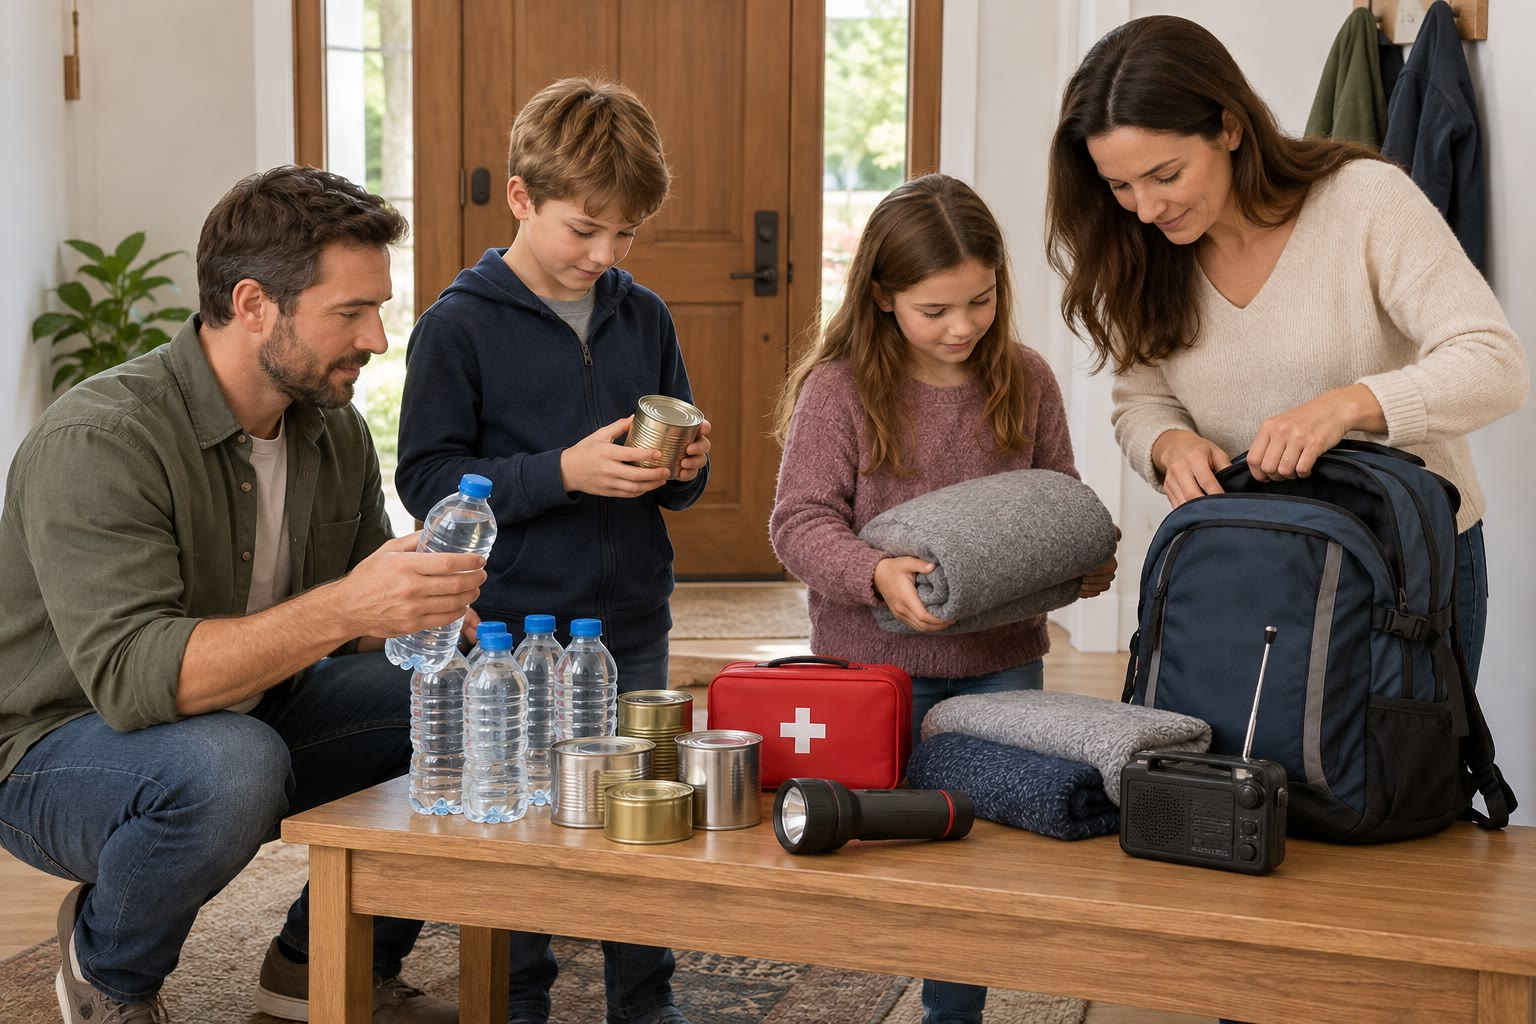
\includegraphics[width=\linewidth]{images/book1/ai/g9-emergency-kit.jpg}
\end{minipage}\hfill
\begin{minipage}[c]{0.52\linewidth}\raggedright
{\small तैयार रहना: एक परिवार अपनी आपातकालीन किट जाँचता है, जो दरवाज़े के पास रखी है,
जल्दी निकलना पड़े तो साथ ले जाने के लिए तैयार: पानी और कई दिनों तक चलने वाला भोजन, एक
टॉर्च, बिजली के बिना चलने वाला एक रेडियो, अतिरिक्त बैटरियाँ, प्राथमिक चिकित्सा किट और गरम
कंबल (एक सामान्य दृश्य का AI
चित्रण)।}
\end{minipage}
% ledger: ready:kit
\label{fig:g9:natural-risks:kit}
\end{omfigure}

\section{ज्वालामुखियों और भ्रंशों पर नज़र}

\omterm{def:g4:volcanoes-earthquakes-first-look:volcano}{ज्वालामुखी} वेधशाला \cref{ch:g7:volcanoes} के चेतावनी संकेतों पर ऐसे उपकरणों से नज़र
रखती है जो दिन-रात चलते हैं और अपने माप वेधशाला को भेजते
हैं।
% ledger: usgs:hvo-toolkit

\begin{omfigure}
\begin{tikzpicture}[x=1cm, y=1cm, font=\footnotesize, >={Stealth[length=2mm]}]
  % ground and cone
  \fill[black!13] (0,0) -- (0,1.0) -- (3.0,1.2) -- (5.4,3.6) -- (6.4,3.6) -- (8.8,1.2) -- (12,1.0) -- (12,0) -- cycle;
  \draw[black!60] (0,1.0) -- (3.0,1.2) -- (5.4,3.6) -- (6.4,3.6) -- (8.8,1.2) -- (12,1.0);
  % magma chamber and conduit
  \fill[omWarm!70] (5.9,0.6) ellipse (1.5 and 0.38);
  \fill[omWarm!70] (5.75,0.9) rectangle (6.05,3.6);
  \node[white, font=\scriptsize\bfseries] at (5.9,0.58) {मैग्मा};
  % gas plume, drifting west
  \fill[black!10] (5.8,3.95) circle (0.3) (5.35,4.35) circle (0.4) (4.75,4.75) circle (0.45);
  % swollen east flank, dashed
  \draw[dashed, omWarm, line width=0.8pt] (6.45,3.7) .. controls (7.5,3.55) and (8.6,2.6) .. (8.85,1.25);
  \draw[->, omWarm] (7.3,2.75) -- (7.7,3.15);
  \node[anchor=west, align=left, text=omWarm!80!black] at (8.2,3.75) {ऊपर उठता मैग्मा\\ ढलान को फुलाता है};
  % tiltmeter on the east flank
  \fill[black] (7.75,2.12) rectangle (8.05,2.24);
  \draw[black!70] (8.1,2.2) -- (8.5,2.45);
  \node[anchor=west, align=left] at (8.5,2.55) {झुकावमापी: फूलने पर\\ ढलान झुकती है};
  % GPS receiver on the west flank, and its satellite
  \draw[black, line width=0.6pt] (4.4,2.6) -- (4.4,2.95);
  \fill[black] (4.25,2.95) rectangle (4.55,3.05);
  \draw[black] (4.4,3.05) circle (0.1);
  \draw[black, fill=white] (1.7,4.85) rectangle (2.0,5.05);
  \draw[black] (1.4,4.95) -- (2.3,4.95);
  \node[anchor=east] at (1.35,4.95) {उपग्रह};
  \draw[black!50, dashed] (4.3,3.15) -- (2.05,4.8);
  \draw[black!70] (3.05,2.65) -- (4.2,2.85);
  \node[anchor=east, align=right] at (3.0,2.6) {GPS अभिग्राही: ज़मीन\\ मिलीमीटरों में\\ खिसकती है};
  % gas instrument on the crater rim
  \fill[black] (6.45,3.6) rectangle (6.75,3.75);
  \draw[black!70] (6.8,3.75) -- (7.1,4.45);
  \node[anchor=west, align=left] at (7.1,4.6) {गैस उपकरण: क्रेटर से\\ निकलती गैसें};
  % seismometer (in the ground)
  \fill[black] (2.1,0.95) rectangle (2.4,1.1);
  \node[anchor=north, align=center] at (1.6,0.85) {भूकंपमापी:\\ छोटे भूकंप};
  % camera, east, looking at the summit
  \fill[black] (10.7,1.12) rectangle (11.0,1.32);
  \fill[black] (10.7,1.17) -- (10.55,1.12) -- (10.55,1.32) -- (10.7,1.27) -- cycle;
  \node[anchor=north, align=center] at (10.8,0.85) {कैमरा:\\ शिखर पर नज़र};
\end{tikzpicture}

{\small \omterm{def:g4:volcanoes-earthquakes-first-look:volcano}{ज्वालामुखी} पर नज़र (एक रेखाचित्र, पैमाने पर नहीं)। \omterm{def:g7:earthquakes:seismometer}{भूकंपमापी} छोटे \omterm{def:g4:volcanoes-earthquakes-first-look:earthquake}{भूकंपों} को
गिनते हैं; \omterm{def:g3:stones-pebbles-sand:rock}{चट्टान} में गड़े झुकावमापी और GPS अभिग्राही मापते हैं कि नीचे \omterm{def:g7:volcanoes:magma}{मैग्मा} इकट्ठा
होने पर ज़मीन कैसे झुकती और खिसकती है; दूसरे उपकरण निकलती गैसों को मापते हैं; कैमरे शिखर
पर नज़र रखते हैं। \omterm{def:g4:clouds-rain-snow:rain-gauge}{वर्षामापी} \omterm{def:g4:volcanoes-earthquakes-first-look:volcano}{ज्वालामुखी} के संकेतों को भारी \omterm{def:g4:clouds-rain-snow:precipitation}{बारिश} के प्रभावों से अलग पहचानने
में मदद करते
हैं।}
% ledger: usgs:hvo-toolkit
\label{fig:g9:natural-risks:monitoring}
\end{omfigure}

इनमें से कोई भी संकेत \omterm{def:g4:volcanoes-earthquakes-first-look:eruption}{उद्गार} का दिन और घंटा नहीं बताता। वैज्ञानिक उन्हें साथ मिलाकर पढ़ते
हैं, जैसे कोई डॉक्टर किसी मरीज़ के कई माप पढ़ता है, और बताते हैं कि ख़तरा कैसे बदल रहा
है; अधिकारी तय करते हैं कि कब कोई इलाक़ा बंद करना है और कब लोगों को वहाँ से निकालना है।
पिनातूबो पर यह कड़ी काम कर गई। नेवाडो देल रुइज़ पर \omterm{def:g4:volcanoes-earthquakes-first-look:volcano}{ज्वालामुखी} एक वर्ष से संकेत दे रहा
था, \omterm{def:g4:volcanoes-earthquakes-first-look:earthquake}{भूकंपों} के झुंडों के साथ, पर उपकरण कम थे, और वैज्ञानिकों से आर्मेरो के लोगों तक की
कड़ी टूटी हुई
थी।
% ledger: usgs:armero, usgs:hvo-toolkit, usgs:pinatubo-1991

\omterm{def:g7:earthquakes:fault}{भ्रंशों} पर भी इसी तरह नज़र रखी जाती है, \omterm{def:g7:earthquakes:seismometer}{भूकंपमापियों} और GPS केंद्रों के जालों से, जो
मिलीमीटर-दर-मिलीमीटर मापते हैं कि \omterm{def:g7:earthquakes:fault}{भ्रंश} के दोनों पक्ष धीरे-धीरे कैसे खिसकते हैं। इससे पता
चलता है कि कौन-से \omterm{def:g7:earthquakes:fault}{भ्रंश} अगले बड़े \omterm{def:g4:volcanoes-earthquakes-first-look:earthquake}{भूकंप} का तनाव जमा कर रहे हैं, पर यह नहीं कि वह कब आएगा।
\omterm{def:g4:volcanoes-earthquakes-first-look:earthquake}{भूकंपों} के लिए \omterm{def:g9:natural-risks:prevention}{रोकथाम} ही मुख्य बचाव
है।
% ledger: usgs:gps, usgs:eq-basics

\section{संकट मानचित्र और बाढ़ क्षेत्र}

\omterm{def:g9:natural-risks:prevention}{रोकथाम} का पहला क़दम यह जानना है कि कोई संकट कहाँ आ सकता है।

\begin{definition}[संकट मानचित्र]\label{def:g9:natural-risks:hazard-map}
\emph{संकट मानचित्र}\index{संकट मानचित्र} वे जगहें दिखाता है जहाँ तक कोई \omterm{def:g5:natural-hazards:hazard}{प्राकृतिक
संकट} पहुँच सकता है, अक्सर ख़तरे के कई स्तरों के साथ। उसे इस आधार पर बनाया जाता है कि
संकट ने अतीत में क्या किया है और ज़मीन का आकार कैसा है।
\end{definition}

इस अध्याय की शुरुआत का नेवाडो देल रुइज़ का \omterm{def:g2:drawing-to-map:map}{मानचित्र} एक \omterm{def:g9:natural-risks:hazard-map}{संकट मानचित्र} है: अतीत के कीचड़
प्रवाह \omterm{def:g1:landscapes-around-us:landform}{घाटियों} के साथ-साथ चले थे, और अगले भी उन्हीं के साथ चलते। \omterm{def:g5:water-shapes-the-land:flood}{बाढ़} के \omterm{def:g2:drawing-to-map:map}{मानचित्र} भी यही
विचार अपनाते हैं। पानी \omterm{def:g1:landscapes-around-us:water}{नदी} के बगल की नीची, समतल ज़मीन पर फैलता है: \omterm{def:g5:water-shapes-the-land:flood}{बाढ़} जितनी ऊँची, वह
ज़मीन की उतनी चौड़ी पट्टी ढकती है। \omterm{def:g5:water-shapes-the-land:flood}{बाढ़} का \omterm{def:g2:drawing-to-map:map}{मानचित्र} किसी चुनी हुई \omterm{def:g5:water-shapes-the-land:flood}{बाढ़} के लिए पानी का किनारा
बनाता है, अक्सर उस \omterm{def:g5:water-shapes-the-land:flood}{बाढ़} के लिए जिसके किसी भी वर्ष में आने या पार होने की संभावना 100 में
1 है। उसे \emph{100-वर्षीय \omterm{def:g5:water-shapes-the-land:flood}{बाढ़}} कहते हैं, पर यह ऐसी \omterm{def:g5:water-shapes-the-land:flood}{बाढ़} नहीं जो सदी में एक बार आए:
वह लगातार दो वर्ष आ सकती
है।
% ledger: fema:flood-zones

\begin{omfigure}
\begin{tikzpicture}
\begin{axis}[axis equal image, xmin=3.5, xmax=7, ymin=2.7, ymax=5.5, width=11.5cm,
  enlargelimits=false, tick label style={font=\scriptsize}, xlabel={पूर्व (km)},
  ylabel={उत्तर (km)}, label style={font=\small}, xtick={3.5,4,...,7}, ytick={3,3.5,...,5.5},
  clip mode=individual]
\addplot[contour] table {figdata/out/grade-9-flood_zone-contours.dat};
\addplot[index contour] table {figdata/out/grade-9-flood_zone-index.dat};
\addplot[fill=omSea, draw=blue!40, line width=0.3pt] table {figdata/out/grade-9-flood_zone-zone10.dat} -- cycle;
\addplot[fill=blue!25, draw=blue!50, line width=0.3pt] table {figdata/out/grade-9-flood_zone-zone.dat} -- cycle;
\addplot[fill=blue!50, draw=none] table {figdata/out/grade-9-flood_zone-zone2.dat} -- cycle;
\addplot[only marks, mark=none, point meta=explicit symbolic, nodes near coords,
  nodes near coords align={center}, nodes near coords style={font=\tiny, fill=white, inner sep=0.6pt, text=omContour}]
  table[meta=z] {figdata/out/grade-9-flood_zone-index-lab.dat};
\addplot[river] table {figdata/out/grade-9-flood_zone-river.dat};
\end{axis}
\end{tikzpicture}

\smallskip
\begin{tikzpicture}[font=\footnotesize]
  \node[anchor=east] at (0,0.125) {नदी से ऊपर बाढ़:};
  \fill[blue!50] (0.2,0) rectangle (0.7,0.25); \node[anchor=west] at (0.8,0.125) {\qty{2}{m}};
  \fill[blue!25, draw=blue!50, line width=0.3pt] (1.9,0) rectangle (2.4,0.25); \node[anchor=west] at (2.5,0.125) {\qty{5}{m}};
  \fill[omSea, draw=blue!40, line width=0.3pt] (3.6,0) rectangle (4.1,0.25); \node[anchor=west] at (4.2,0.125) {\qty{10}{m}};
\end{tikzpicture}

{\small वार्डन पहाड़ियों की \omterm{def:g1:landscapes-around-us:water}{नदी} का \omterm{def:g5:water-shapes-the-land:flood}{बाढ़ का मैदान}, \omterm{def:g1:landscapes-around-us:water}{नदी} पूर्व की ओर बहती है। हर छाया वह
ज़मीन है जिसे \omterm{def:g5:water-shapes-the-land:flood}{बाढ़} ढक लेती अगर वह \omterm{def:g1:landscapes-around-us:water}{नदी} के सामान्य स्तर से 2, 5 या \qty{10}{m} ऊपर उठती:
हर क्षेत्र में छोटे क्षेत्र शामिल हैं। क्षेत्र संकरे रहते हैं क्योंकि \omterm{def:g1:landscapes-around-us:landform}{घाटी} के किनारे उसके
समतल तल से जल्दी ऊपर उठते हैं। पतली रेखाएँ एक ही ऊँचाई के बिंदुओं को जोड़ती हैं, हर
\qty{10}{m} पर, हर \qty{50}{m} पर अंकित; ऐसे \omterm{def:g2:drawing-to-map:map}{मानचित्र} \cref{ch:g9:maps-of-the-earth}
का विषय
हैं।}
% ledger: (invented region: figdata/grade-9/flood_zone.py, parts zone2, zone, zone10)
\label{fig:g9:natural-risks:flood-zones}
\end{omfigure}

\begin{method}[बाढ़ क्षेत्र का मानचित्र पढ़ना]
\begin{enumerate}
  \item पता करो कि क्षेत्र किस \omterm{def:g5:water-shapes-the-land:flood}{बाढ़} को दिखाता है: \omterm{def:g1:landscapes-around-us:water}{नदी} से कितनी ऊपर, या कितनी बार वह
        आ सकती है।
  \item मापनी-पट्टी या जाली की मदद से \omterm{def:g2:drawing-to-map:map}{मानचित्र} पर जगह ढूँढो।
  \item अगर जगह छायांकित क्षेत्र के अंदर है, तो वह \omterm{def:g5:water-shapes-the-land:flood}{बाढ़} उस तक पहुँचेगी; अगर बाहर है,
        तो वह उस \omterm{def:g5:water-shapes-the-land:flood}{बाढ़} में सूखी रहेगी, हर \omterm{def:g5:water-shapes-the-land:flood}{बाढ़} में
        नहीं।
  \item जगहों की तुलना करने के लिए \omterm{def:g1:landscapes-around-us:water}{नदी} से उनकी ऊँचाइयों का उपयोग करो: जितनी नीची,
        उतनी ज़्यादा बार डूबती है।
\end{enumerate}
\end{method}

\begin{example}[नदी के बगल में तीन घर]
ऊपर जैसे किसी \omterm{def:g2:drawing-to-map:map}{मानचित्र} पर एक घर \omterm{def:g1:landscapes-around-us:water}{नदी} से \qty{3}{m} ऊपर की ज़मीन पर खड़ा है। \omterm{def:g1:landscapes-around-us:water}{नदी} से
\qty{2}{m} ऊपर की \omterm{def:g5:water-shapes-the-land:flood}{बाढ़} उस तक नहीं पहुँचती; 5 और \qty{10}{m} की \omterm{def:g5:water-shapes-the-land:flood}{बाढ़ें} पहुँचती हैं।
दूसरा घर, \omterm{def:g1:landscapes-around-us:water}{नदी} से \qty{8}{m} ऊपर, केवल \qty{10}{m} की \omterm{def:g5:water-shapes-the-land:flood}{बाढ़} से घिरता है, और तीसरा, \omterm{def:g1:landscapes-around-us:water}{नदी}
से \qty{30}{m} ऊपर एक ढलान पर, तीनों में से किसी से नहीं। पहला घर सबसे सुभेद्य है:
छोटी \omterm{def:g5:water-shapes-the-land:flood}{बाढ़ें}, जो ज़्यादा बार आती हैं, उस तक पहुँचने के लिए काफ़ी
हैं।
\end{example}

\section{भूकंप झेलने वाले भवन बनाना}

\omterm{def:g4:volcanoes-earthquakes-first-look:earthquake}{भूकंप} में ज़मीन किसी इमारत के नीचे आगे-पीछे खिसकती है, और इमारत नीचे से हिलाई जाती है;
प्रबल \omterm{def:g4:volcanoes-earthquakes-first-look:earthquake}{भूकंप} में ख़तरा सबसे बढ़कर उन इमारतों से आता है जो दरकती और गिरती हैं। इंजीनियर
हिलना रोक नहीं सकते, पर वे ऐसे निर्माण कर सकते हैं कि ढाँचा बिना गिरे हिलने के बलों को
झेल ले।
% ledger: iris:better-wall

\begin{omfigure}
\begin{tikzpicture}[x=1cm, y=1cm, font=\footnotesize, >={Stealth[length=2mm]}]
  % panel 1: a frame that leans
  \begin{scope}
    \fill[black!13] (-0.3,-0.25) rectangle (3.0,0);
    \draw[black!35, dashed] (0.2,0) rectangle (2.5,2.6);
    \draw[black, line width=1.2pt] (0.2,0) -- (0.75,2.6) -- (3.05,2.6) -- (2.5,0);
    \draw[black, line width=1.2pt] (0.47,1.3) -- (2.77,1.3);
    \draw[<->] (0.2,-0.45) -- (1.0,-0.45);
    \node[align=center, anchor=north] at (1.35,-0.65) {(क) नंगा ढाँचा झुक\\ जाता है और गिर सकता है};
  \end{scope}
  % panel 2: braces
  \begin{scope}[xshift=3.7cm]
    \fill[black!13] (-0.3,-0.25) rectangle (3.0,0);
    \draw[black, line width=1.2pt] (0.2,0) rectangle (2.5,2.6);
    \draw[black, line width=1.2pt] (0.2,1.3) -- (2.5,1.3);
    \draw[omWarm, line width=1pt] (0.2,0) -- (2.5,1.3) (2.5,0) -- (0.2,1.3)
                                  (0.2,1.3) -- (2.5,2.6) (2.5,1.3) -- (0.2,2.6);
    \node[align=center, anchor=north] at (1.35,-0.65) {(ख) तिरछे टेक\\ उसका आकार बनाए रखते हैं};
  \end{scope}
  % panel 3: shear wall
  \begin{scope}[xshift=7.4cm]
    \fill[black!13] (-0.3,-0.25) rectangle (3.0,0);
    \draw[black, line width=1.2pt] (0.2,0) rectangle (2.5,2.6);
    \draw[black, line width=1.2pt] (0.2,1.3) -- (2.5,1.3);
    \fill[omWarm!35] (1.6,0) rectangle (2.5,2.6);
    \draw[black, line width=0.6pt] (1.6,0) rectangle (2.5,2.6);
    \node[align=center, anchor=north] at (1.35,-0.65) {(ग) ऊपर से नीचे तक एक\\ कठोर अपरूपण दीवार};
  \end{scope}
  % panel 4: base isolation
  \begin{scope}[xshift=11.1cm]
    \fill[black!13] (-0.3,-0.25) rectangle (3.0,0);
    \foreach \x in {0.35,1.35,2.35} \fill[omSea, draw=black!60, rounded corners=1pt] (\x-0.18,0) rectangle (\x+0.18,0.3);
    \draw[black, line width=1.2pt] (0.15,0.3) -- (2.55,0.3);
    \draw[black, line width=1.2pt] (0.2,0.3) rectangle (2.5,2.7);
    \draw[black, line width=1.2pt] (0.2,1.5) -- (2.5,1.5);
    \draw[<->] (0.2,-0.45) -- (1.0,-0.45);
    \node[align=center, anchor=north] at (1.35,-0.65) {(घ) विलगक ज़मीन को\\ नीचे खिसकने देते हैं};
  \end{scope}
\end{tikzpicture}

{\small एक ही ज़मीन से हिलाए गए चार ढाँचे (एक रेखाचित्र)। केवल खंभों और धरनों का ढाँचा
झुककर ढह सकता है (क)। तिरछे टेक (ख) और कठोर अपरूपण दीवारें (ग) उसे झुकने से रोकती हैं;
धरनों और खंभों के बीच मज़बूत जोड़ उसे एक साथ थामे रखते हैं। इमारत के नीचे रखे विलगक (घ)
ज़मीन के खिसकने पर लचक जाते हैं, ताकि गति का बहुत कम हिस्सा इमारत तक
पहुँचे।}
% ledger: iris:better-wall, explo:base-isolation
\label{fig:g9:natural-risks:buildings}
\end{omfigure}

यही सिद्धांत किसी घर, स्कूल या पुल के काम आते हैं। इन्हें लागू करना तब सबसे आसान है जब
इमारत की रूपरेखा बनाई जा रही हो, न कि बाद में किसी पुरानी इमारत में जोड़ते
समय।

\begin{inthelab}[हिलती ट्रे पर एक मीनार]
घर के अंदर, पीने की नलियों या लकड़ी की तीलियों और मॉडलिंग क्ले से एक ही ऊँचाई की दो छोटी
मीनारें बनाओ, दो मंज़िला ढाँचों के रूप में। दूसरी को हर ओर तिरछे टेक दो। दोनों को एक ट्रे
पर खड़ा करो, फिर ट्रे को तेज़ी से आगे-पीछे खिसकाओ, पहले धीरे, फिर ज़ोर से। कौन-सी मीनार
पहले झुकती है? कौन-सी अपना आकार बनाए रखती है? फिर नंगी मीनार को एक हल्के कार्ड के नीचे
चार कंचों पर रखो, और फिर से हिलाओ: क्या बदलता
है?
\end{inthelab}

\section{समय पर चेतावनियाँ}

\omterm{def:g9:natural-risks:prevention}{रोकथाम} का आख़िरी हिस्सा चेतावनी है। \omterm{def:g7:earthquakes:tsunami}{सुनामियों} के लिए यह \omterm{def:g2:water-on-earth:ocean}{महासागर} के तल पर शुरू होती है।
उन जगहों के पास जहाँ विनाशकारी \omterm{def:g7:earthquakes:tsunami}{सुनामियाँ} पहले शुरू हुई हैं, समुद्री तल पर एक दाब अभिलेखी
रखा होता है जो हर \qty{15}{s} पर अपने ऊपर के पानी का भार पढ़ता है, जिससे \omterm{def:g2:water-on-earth:ocean}{समुद्र} की सतह
की ऊँचाई मिलती है। वह अपने माप पानी में से ध्वनि के ज़रिए सतह पर बँधे एक प्लव को भेजता है,
और प्लव उन्हें उपग्रह से \omterm{def:g7:earthquakes:tsunami}{सुनामी} चेतावनी केंद्रों तक पहुँचाता है। किसी भी \omterm{def:g1:landscapes-around-us:water}{तट} से दूर \omterm{def:g2:water-on-earth:ocean}{समुद्र}
का उठना रास्ते में आती \omterm{def:g7:earthquakes:tsunami}{सुनामी} दिखाता है, दूर के तटों तक उसके पहुँचने से घंटों
पहले।
% ledger: ndbc:dart, nws:tsunami-speed

\begin{omfigure}
\begin{minipage}[c]{0.4\linewidth}\centering
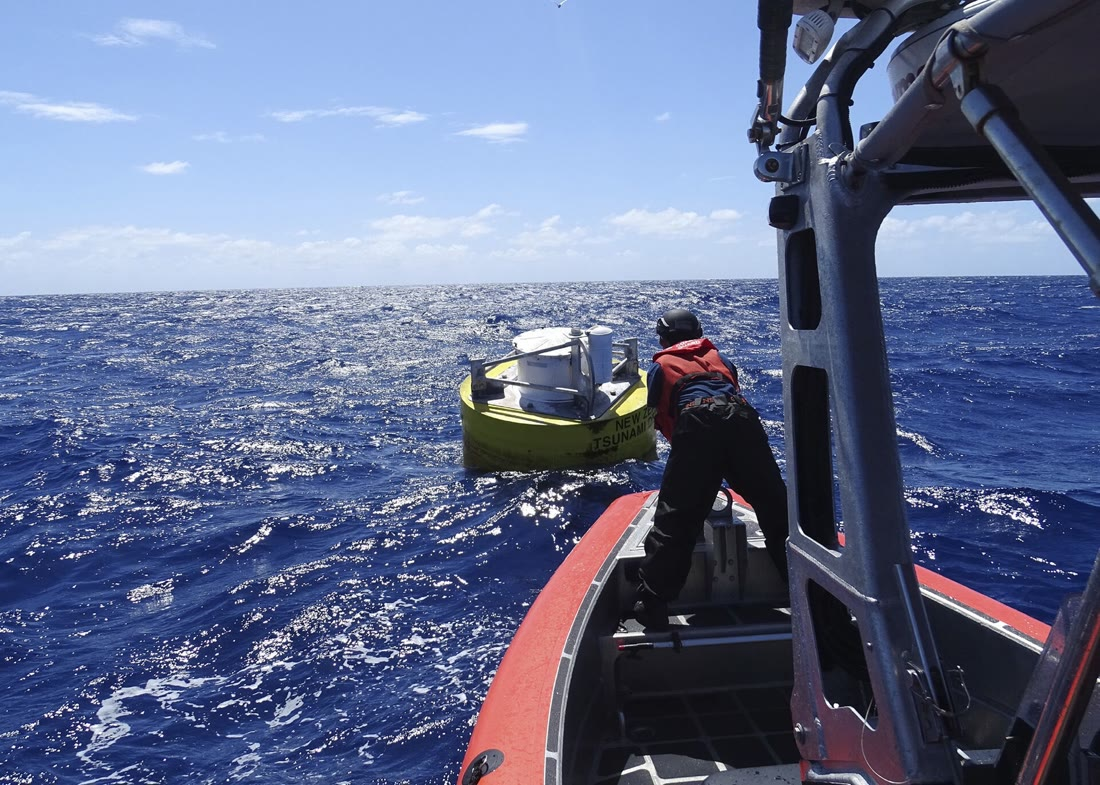
\includegraphics[width=\linewidth]{images/book1/g9-dart-buoy.jpg}
\end{minipage}\hfill
\begin{minipage}[c]{0.56\linewidth}\raggedright
{\small संयुक्त राज्य तटरक्षक बल के एक जहाज़ का एक दल-सदस्य, नवंबर 2021 में, प्रशांत
\omterm{def:g2:water-on-earth:ocean}{महासागर} में एक \omterm{def:g7:earthquakes:tsunami}{सुनामी} चेतावनी प्लव का निरीक्षण करता है। प्लव हज़ारों मीटर नीचे समुद्री तल
पर रखे एक दाब अभिलेखी के ऊपर तैरता है। अमेरिकी तटरक्षक बल (सार्वजनिक डोमेन, विकिमीडिया
कॉमन्स के ज़रिए)।}
\end{minipage}
% ledger: commons:dart-buoy
\label{fig:g9:natural-risks:buoy}
\end{omfigure}

\begin{history}[प्लवों का एक जाल]
2001 में प्रशांत \omterm{def:g2:water-on-earth:ocean}{महासागर} में ऐसे छह केंद्रों की पहली शृंखला पूरी हुई। दिसंबर 2004 की
\omterm{def:g7:earthquakes:tsunami}{सुनामी} के बाद, जो बिना किसी चेतावनी प्रणाली के हिंद \omterm{def:g2:water-on-earth:ocean}{महासागर} के तटों तक पहुँची थी
(\cref{ch:g7:earthquakes}), जाल बढ़ा: मार्च 2008 तक 39 केंद्र
थे।
\end{history}
% ledger: ndbc:dart

चेतावनी तभी जानें बचाती है जब वह ऐसे लोगों तक पहुँचे जो जानते हैं कि उसके साथ क्या करना
है: ऊँची ज़मीन तक के रास्तों पर निशान लगे हैं और उनका अभ्यास हुआ है, आपातकालीन किट तैयार
है, स्कूल अभ्यास करवाते हैं। आर्मेरो में संकट ज्ञात था और \omterm{def:g2:drawing-to-map:map}{मानचित्र} बन चुका था; चेतावनी
कभी कस्बे तक नहीं पहुँची।
% ledger: ready:kit, usgs:armero

\section{अभ्यास}

\begin{exercise}[$\star$]\label{exo:g9:natural-risks:1}
संकट या \omterm{def:g9:natural-risks:vulnerability}{सुभेद्यता}? (क) एक \omterm{def:g1:landscapes-around-us:water}{नदी} जिसमें लगभग हर वसंत \omterm{def:g5:water-shapes-the-land:flood}{बाढ़} आती है। (ख) बिना चेतावनी प्रणाली
का एक गाँव। (ग) बिना ढाँचे के ईंट के भारी घर। (घ) पास के एक \omterm{def:g7:earthquakes:fault}{भ्रंश} पर प्रबल \omterm{def:g4:volcanoes-earthquakes-first-look:earthquake}{भूकंप}।
(ङ) एक \omterm{def:g1:landscapes-around-us:landform}{घाटी} के \omterm{def:g5:water-shapes-the-land:source-mouth}{मुहाने} पर बसा कस्बा जहाँ पहले कीचड़ प्रवाह बह चुके
हैं।
\end{exercise}

\begin{exercise}[$\star$]\label{exo:g9:natural-risks:2}
सही या ग़लत? ग़लत वाक्यों को सुधारो। (क) ऐसी जगह पर \omterm{def:g5:natural-hazards:hazard}{प्राकृतिक संकट} जहाँ कोई नहीं रहता,
ऊँचा \omterm{def:g9:natural-risks:risk}{जोखिम} है। (ख) \omterm{def:g9:natural-risks:prevention}{रोकथाम} किसी कस्बे की \omterm{def:g9:natural-risks:vulnerability}{सुभेद्यता} घटा सकती है। (ग) \omterm{def:g9:natural-risks:hazard-map}{संकट मानचित्र} दिखाता
है कि संकट कहाँ आ सकता है। (घ) एक अच्छी चेतावनी प्रणाली \omterm{def:g4:volcanoes-earthquakes-first-look:volcano}{ज्वालामुखी} को कम ख़तरनाक बना
देती है।
\end{exercise}

\begin{exercise}[$\star$]\label{exo:g9:natural-risks:3}
हर संकट के लिए बताओ कि क्या उसका पूर्वानुमान दिनों या घंटों पहले हो सकता है: (क) \omterm{def:g5:natural-hazards:storm}{तूफ़ान};
(ख) भारी \omterm{def:g4:clouds-rain-snow:precipitation}{बारिश} के बाद \omterm{def:g5:water-shapes-the-land:flood}{बाढ़}; (ग) \omterm{def:g4:volcanoes-earthquakes-first-look:earthquake}{भूकंप}; (घ) किसी \omterm{def:g1:landscapes-around-us:water}{तट} पर, उसके शुरू होने की जगह से दूर,
\omterm{def:g7:earthquakes:tsunami}{सुनामी} का आगमन।
\end{exercise}

\begin{exercise}[$\star$]\label{exo:g9:natural-risks:4}
% ledger: usgs:hvo-toolkit
जिस \omterm{def:g4:volcanoes-earthquakes-first-look:volcano}{ज्वालामुखी} पर नज़र रखी जाती है उसका चित्र देखो। हर उपकरण क्या मापता है, और वह \omterm{def:g4:volcanoes-earthquakes-first-look:eruption}{उद्गार}
के किस चेतावनी संकेत पर नज़र रखता है? (क) \omterm{def:g7:earthquakes:seismometer}{भूकंपमापी}। (ख) झुकावमापी। (ग) GPS अभिग्राही।
(घ) गैस उपकरण।
\end{exercise}

\begin{exercise}[$\star\star$]\label{exo:g9:natural-risks:5}
% ledger: usgs:armero
1985 में नेवाडो देल रुइज़ के कीचड़ प्रवाह \qty{45}{km} दूर आर्मेरो तक \omterm{def:g4:volcanoes-earthquakes-first-look:eruption}{उद्गार} के लगभग
दो घंटे बाद पहुँचे। (क) किलोमीटर प्रति घंटे में उनकी औसत चाल क्या थी? (ख) कोई व्यक्ति
लगभग \qty{4}{km/h} से चलता है। दो घंटे में लोग कितनी दूर पैदल जा सकते थे? (ग) वे
निकले क्यों नहीं? (घ) दो ऐसी चीज़ें बताओ जो उन्हें बचा सकती
थीं।
\end{exercise}

\begin{exercise}[$\star\star$]\label{exo:g9:natural-risks:6}
% ledger: (invented region: figdata/grade-9/flood_zone.py)
वार्डन पहाड़ियों का \omterm{def:g5:water-shapes-the-land:flood}{बाढ़} क्षेत्र \omterm{def:g2:drawing-to-map:map}{मानचित्र} उपयोग करो। (क) कौन-सी \omterm{def:g5:water-shapes-the-land:flood}{बाढ़} सबसे चौड़ी पट्टी ढकती
है? (ख) \omterm{def:g2:drawing-to-map:map}{मानचित्र} की जाली से \qty{5}{km} पूर्व पर \omterm{def:g1:landscapes-around-us:landform}{घाटी} में हर क्षेत्र की चौड़ाई
मापो। (ग) एक खलिहान \omterm{def:g1:landscapes-around-us:water}{नदी} से \qty{6}{m} ऊपर की ज़मीन पर खड़ा है। तीनों में से कौन-सी
\omterm{def:g5:water-shapes-the-land:flood}{बाढ़ें} उस तक पहुँचती हैं? (घ) \omterm{def:g1:landscapes-around-us:water}{नदी} से \qty{2}{m} ऊपर की \omterm{def:g5:water-shapes-the-land:flood}{बाढ़} ही सबसे ज़्यादा बार क्यों
आती
है?
\end{exercise}

\begin{exercise}[$\star\star$]\label{exo:g9:natural-risks:7}
हर स्थिति को \omterm{def:g9:natural-risks:risk}{जोखिम} की जाली पर रखो (कम या ऊँचा संकट, कम या ऊँची \omterm{def:g9:natural-risks:vulnerability}{सुभेद्यता}) और बताओ कि
\omterm{def:g9:natural-risks:risk}{जोखिम} कम, मध्यम या ऊँचा है। (क) एक सक्रिय \omterm{def:g7:earthquakes:fault}{भ्रंश} पर बसे कस्बे में मज़बूत इमारतें और अभ्यास।
(ख) ऐसी \omterm{def:g1:landscapes-around-us:water}{नदी} के \omterm{def:g5:water-shapes-the-land:flood}{बाढ़} के \omterm{def:g1:landscapes-around-us:landform}{मैदान} पर एक शिविर स्थल जिसमें शायद ही कभी \omterm{def:g5:water-shapes-the-land:flood}{बाढ़} आती है। (ग) एक
सक्रिय \omterm{def:g4:volcanoes-earthquakes-first-look:volcano}{ज्वालामुखी} के तल पर कमज़ोर घरों वाला एक गाँव, बिना किसी वेधशाला के। (घ) किसी भी
\omterm{def:g7:earthquakes:fault}{भ्रंश}, \omterm{def:g1:landscapes-around-us:water}{नदी} या \omterm{def:g4:volcanoes-earthquakes-first-look:volcano}{ज्वालामुखी} से दूर एक \omterm{def:g1:landscapes-around-us:landform}{पहाड़ी} की चोटी पर बसा कस्बा।
\end{exercise}

\begin{exercise}[$\star\star$]\label{exo:g9:natural-risks:8}
% ledger: iris:better-wall, explo:base-isolation
तीन स्कूल एक ही ज़मीन पर बने हैं। स्कूल A खंभों और धरनों का एक ढाँचा है जिनके बीच ईंट की
दीवारें हैं; स्कूल B में वही ढाँचा तिरछे टेकों और दो अपरूपण दीवारों के साथ है; स्कूल C में
B का ढाँचा है, विलगकों पर खड़ा। (क) \omterm{def:g4:volcanoes-earthquakes-first-look:earthquake}{भूकंप} में उन्हें सबसे सुरक्षित से सबसे कम सुरक्षित के
क्रम में रखो। (ख) समझाओ कि टेक क्या करते हैं। (ग) समझाओ कि विलगक क्या करते
हैं।
\end{exercise}

\begin{exercise}[$\star\star$]\label{exo:g9:natural-risks:9}
% ledger: fema:flood-zones
एक \omterm{def:g5:water-shapes-the-land:flood}{बाढ़} \omterm{def:g2:drawing-to-map:map}{मानचित्र} 100-वर्षीय \omterm{def:g5:water-shapes-the-land:flood}{बाढ़} दिखाता है, जिसके किसी भी वर्ष में आने या पार होने की
संभावना 100 में 1 है। (क) इस संभावना को प्रतिशत में लिखो। (ख) एक पड़ोसी कहता है:
``100-वर्षीय \omterm{def:g5:water-shapes-the-land:flood}{बाढ़} पिछले वर्ष आई थी, इसलिए हम 99 वर्षों तक सुरक्षित हैं।'' क्या ग़लत है?
(ग) औसतन, 300 वर्षों में ऐसी कितनी \omterm{def:g5:water-shapes-the-land:flood}{बाढ़ें}
आएँगी?
\end{exercise}

\begin{exercise}[$\star\star$]\label{exo:g9:natural-risks:10}
% ledger: ndbc:dart, nws:tsunami-speed
एक \omterm{def:g7:earthquakes:tsunami}{सुनामी} चेतावनी केंद्र हर \qty{15}{s} पर समुद्री तल का दाब पढ़ता है। (क) एक घंटे
में वह कितने माप लेता है? (ख) 365 दिनों के एक वर्ष में? जवाब वैज्ञानिक संकेतन में
लिखो। (ग) \omterm{def:g7:earthquakes:tsunami}{सुनामी} गहरे \omterm{def:g2:water-on-earth:ocean}{महासागर} को लगभग \qty{800}{km/h} से पार करती है।
\qty{2400}{km} दूर के \omterm{def:g1:landscapes-around-us:water}{तट} तक पहुँचने में उसे कितना समय लगता है? (घ) वह समय क्यों मायने
रखता है?
\end{exercise}

\begin{exercise}[$\star\star\star$]\label{exo:g9:natural-risks:11}
% ledger: ready:kit
चार लोगों का एक परिवार 3 दिनों के पानी के साथ एक आपातकालीन किट तैयार करता है, प्रति व्यक्ति
प्रति दिन लगभग \qty{3.8}{L}, पीने और धोने के लिए। (क) उन्हें कितने लीटर पानी चाहिए?
(ख) यह \qty{1.5}{L} की कितनी बोतलें है? (ग) किट में रखी चार दूसरी चीज़ों के नाम बताओ,
और बताओ कि हर एक क्यों काम की है। (घ) किट दरवाज़े के पास क्यों रखी जाती
है?
\end{exercise}

\begin{exercise}[$\star\star\star$]\label{exo:g9:natural-risks:12}
% ledger: usgs:armero, usgs:hvo-toolkit
एक कस्बा एक \omterm{def:g1:landscapes-around-us:water}{नदी} के बगल में, बर्फ़ से ढके एक \omterm{def:g4:volcanoes-earthquakes-first-look:volcano}{ज्वालामुखी} से नीचे आने वाली \omterm{def:g1:landscapes-around-us:landform}{घाटी} के \omterm{def:g5:water-shapes-the-land:source-mouth}{मुहाने} पर
बसा है। उसकी गलियों के नीचे पुराने कीचड़ प्रवाहों के निक्षेप हैं। \omterm{def:g4:volcanoes-earthquakes-first-look:volcano}{ज्वालामुखी} छोटे \omterm{def:g4:volcanoes-earthquakes-first-look:earthquake}{भूकंपों} के
साथ काँपने लगा है। कस्बे के लिए पाँच बिंदुओं की एक \omterm{def:g9:natural-risks:prevention}{रोकथाम} योजना लिखो। हर बिंदु के लिए
बताओ कि वह \omterm{def:g9:natural-risks:risk}{जोखिम} की संकट वाली ओर (संकट को जानना और उस पर नज़र रखना) काम करता है या
\omterm{def:g9:natural-risks:vulnerability}{सुभेद्यता} वाली
ओर।
\end{exercise}

\section{समस्या: नया स्कूल कहाँ बने?}

\begin{problem}[{सप्ताहांत समस्या --- वार्डन पहाड़ियों के मानचित्र पर बाढ़ों, खड़ी ढलानों
और भ्रंश से दूर एक नया स्कूल रखा जाता है; अंतिम उत्तर बाढ़ क्षेत्र के अंदर के घरों की
संख्या है}]
\label{pb:g9:natural-risks:1}
% ledger: (invented region: figdata/grade-9/flood_zone.py: sites A, B, C; 17 of 28 houses in the 5 m zone)
वार्डन पहाड़ियों के गाँव को एक नए स्कूल की ज़रूरत है, और तीन जगहें प्रस्तावित हैं: A, B और C,
नीचे के \omterm{def:g2:drawing-to-map:map}{मानचित्र} पर। \omterm{def:g2:drawing-to-map:map}{मानचित्र} पर छायांकित \omterm{def:g5:water-shapes-the-land:flood}{बाढ़} क्षेत्र \omterm{def:g1:landscapes-around-us:water}{नदी} से \qty{5}{m} से कम ऊँची सारी
ज़मीन है, जिसे एक बड़ी \omterm{def:g5:water-shapes-the-land:flood}{बाढ़} ढक लेती। तालिका हर जगह के लिए ज़मीन की ऊँचाई, उसके बगल में \omterm{def:g1:landscapes-around-us:water}{नदी}
का स्तर, और ढलान पर क्षैतिज मापे गए \qty{200}{m} पर ज़मीन कितनी ऊपर उठती है, यह
देती
है।

\begin{center}
{\small
\begin{tabular}{|c|c|c|c|}
\hline
जगह & ज़मीन की ऊँचाई & बगल में \omterm{def:g1:landscapes-around-us:water}{नदी} का स्तर & \qty{200}{m} पर ज़मीन का उठाव \\
\hline
A & \qty{137}{m} & \qty{137}{m} & \qty{1.4}{m} \\
B & \qty{276}{m} & \qty{126}{m} & \qty{83}{m} \\
C & \qty{236}{m} & \qty{143}{m} & \qty{20}{m} \\
\hline
\end{tabular}}
\end{center}

\begin{omfigure}
\begin{tikzpicture}
\begin{axis}[axis equal image, xmin=3.5, xmax=7, ymin=2.7, ymax=5.5, width=11.5cm,
  enlargelimits=false, tick label style={font=\scriptsize}, xlabel={पूर्व (km)},
  ylabel={उत्तर (km)}, label style={font=\small}, xtick={3.5,4,...,7}, ytick={3,3.5,...,5.5}]
\addplot[contour] table {figdata/out/grade-9-flood_zone-contours.dat};
\addplot[index contour] table {figdata/out/grade-9-flood_zone-index.dat};
\addplot[fill=blue!25, draw=blue!50, line width=0.3pt] table {figdata/out/grade-9-flood_zone-zone.dat} -- cycle;
\addplot[only marks, mark=none, point meta=explicit symbolic, nodes near coords,
  nodes near coords align={center}, nodes near coords style={font=\tiny, fill=white, inner sep=0.6pt, text=omContour}]
  table[meta=z] {figdata/out/grade-9-flood_zone-index-lab.dat};
\addplot[river] table {figdata/out/grade-9-flood_zone-river.dat};
\addplot[fault] table {figdata/out/shared-region-fault.dat};
\addplot[only marks, mark=square*, mark size=1.5pt, mark options={fill=black}] table {figdata/out/grade-9-flood_zone-houses-in.dat};
\addplot[only marks, mark=square*, mark size=1.5pt, mark options={fill=black}] table {figdata/out/grade-9-flood_zone-houses-out.dat};
\addplot[only marks, mark=*, mark size=2.6pt, mark options={fill=omWarm, draw=black}, point meta=explicit symbolic,
  nodes near coords, nodes near coords align={anchor=south west},
  nodes near coords style={font=\small\bfseries, fill=white, inner sep=1pt, xshift=2.5pt, yshift=2.5pt}]
  table[meta=name] {figdata/out/grade-9-flood_zone-sites.dat};
\node[font=\footnotesize, fill=white, inner sep=1pt, anchor=west] at (axis cs:6.42,5.05) {भ्रंश};
\coordinate (na) at (axis cs:3.7,4.75);
\fill[black] (axis cs:5.8,2.85) rectangle (axis cs:5.925,2.9);
\fill[white] (axis cs:5.925,2.85) rectangle (axis cs:6.05,2.9);
\fill[black] (axis cs:6.05,2.85) rectangle (axis cs:6.175,2.9);
\fill[white] (axis cs:6.175,2.85) rectangle (axis cs:6.3,2.9);
\draw[black, line width=0.4pt] (axis cs:5.8,2.85) rectangle (axis cs:6.3,2.9);
\node[font=\footnotesize, above, inner sep=1.5pt, fill=white] at (axis cs:6.05,2.9) {\qty{500}{m}};
\end{axis}
\fill[white, opacity=0.85] ($(na)+(-0.35,-0.1)$) rectangle ($(na)+(0.35,1.45)$);
\pic at (na) {northarrow};
\end{tikzpicture}

{\small गाँव, स्कूल की तीन जगहें और \omterm{def:g5:water-shapes-the-land:flood}{बाढ़} क्षेत्र (छायांकित), वार्डन पहाड़ियों के \omterm{def:g2:drawing-to-map:map}{मानचित्र}
पर (बराबर ऊँचाई की पतली रेखाएँ हर \qty{10}{m} पर)। हर छोटा काला वर्ग एक घर है। मोटी
काली रेखा एक \omterm{def:g7:earthquakes:fault}{भ्रंश}
है।}
\label{fig:g9:natural-risks:school-map}
\end{omfigure}

\noindent\textbf{भाग I --- बाढ़ क्षेत्र।}\par\nopagebreak
\begin{enumerate}[beginpenalty=10000]
  \item तालिका के \omterm{def:g1:landscapes-around-us:water}{नदी} स्तरों से बताओ कि \omterm{def:g1:landscapes-around-us:water}{नदी} किस ओर बहती
        है।
  \item हर जगह की ऊँचाई उसके बगल की \omterm{def:g1:landscapes-around-us:water}{नदी} से ऊपर निकालो।
  \item तीनों में से कौन-सी जगह \omterm{def:g5:water-shapes-the-land:flood}{बाढ़} क्षेत्र में है?
  \item मापनी-पट्टी से जगह A पर \omterm{def:g1:landscapes-around-us:landform}{घाटी} में \omterm{def:g5:water-shapes-the-land:flood}{बाढ़} क्षेत्र की चौड़ाई
        मापो।
\end{enumerate}

\noindent\textbf{भाग II --- ढलानें और भ्रंश।}\par\nopagebreak
\begin{enumerate}[resume, beginpenalty=10000]
  \item प्रतिशत में ढलान, समतल मापे गए हर \qty{100}{m} पर ज़मीन का उठाव है। हर जगह
        पर ढलान निकालो।
  \item कौन-सी जगह \omterm{def:g5:natural-hazards:landslide}{भूस्खलन} के ख़तरे में होगी? समझाओ।
  \item मापनी-पट्टी से हर जगह से \omterm{def:g7:earthquakes:fault}{भ्रंश} तक की दूरी का अनुमान
        लगाओ।
  \item मान लो कि \omterm{def:g7:earthquakes:fault}{भ्रंश} अब भी खिसक सकता है। उसके ठीक ऊपर की ज़मीन स्कूल के लिए बुरी
        जगह क्यों है?
\end{enumerate}

\noindent\textbf{भाग III --- चुनाव।}\par\nopagebreak
\begin{enumerate}[resume, beginpenalty=10000]
  \item हर जगह की एक पंक्ति और तीन स्तंभों वाली एक तालिका बनाओ: \omterm{def:g5:water-shapes-the-land:flood}{बाढ़} क्षेत्र में?
        खड़ी ढलान? \omterm{def:g7:earthquakes:fault}{भ्रंश} पर? उसे हाँ या नहीं से भरो।
  \item तुम कौन-सी जगह चुनोगे? तालिका से अपना चुनाव सही ठहराओ।
  \item चुनी गई जगह अब भी ऐसे क्षेत्र में है जहाँ ज़मीन हिल सकती है। स्कूल बनाने के दो
        तरीक़े, और उसके छात्रों की एक आदत, बताओ जो उसकी \omterm{def:g9:natural-risks:vulnerability}{सुभेद्यता} घटाते
        हैं।
  \item स्कूल \omterm{def:g5:water-shapes-the-land:flood}{बाढ़} के समय आश्रय का काम भी करेगा। गाँव के उन घरों को गिनो जो \omterm{def:g5:water-shapes-the-land:flood}{बाढ़} क्षेत्र के
        अंदर खड़े हैं। यह सभी घरों का कितना भाग है?
\end{enumerate}
\end{problem}
